
\chapter{图片匹配}

\section{LOGO匹配}

在商标识别中,我们实现的功能为用户上传一张图片,返回最匹配的商标的名称。我们建立了一个商标的图片库(logo\_recognition/logo\_images)以及一个商标索引(brands.txt),对每张上传的图片,逐一与图片库中的图片比较sift特征向量,每个品牌的得分为该品牌下每张图片与待测图片的匹配特征点个数的平均值,最后返回得分最高的品牌。

特征点的选择以及特征向量的计算使用opencv库中的SIFT\_create.detectAndCompute函数。

\begin{python}
detector = cv2.xfeatures2d.SIFT_create() # 特征向量计算使用sift算法
QueryImgBGR=cv2.imread(img)
QueryImg=cv2.cvtColor(QueryImgBGR,cv2.COLOR_BGR2GRAY) # 读取图片灰度图
QueryImg = cv2.GaussianBlur(QueryImg, (3, 3), 0) # 高斯模糊,降点噪点影响
queryKP,queryDesc=detector.detectAndCompute(QueryImg,None) # queryKP,queryDesc为特征点坐标以及特征向量的列表
\end{python}

我们使用FlannBasedMatcher寻找最近邻近似匹配,使用knnmatch匹配处理,返回匹配的特征点对,当两特征值的欧式距离小于一定值时视为匹配成功。

\begin{python}
scores = []
flannParam = dict(algorithm = 0,tree = 5)
flann = cv2.FlannBasedMatcher(flannParam,{}) # 最近邻近似匹配

for brand in brands:
    trainImg = []
    score = 0.0
    for filename in glob.glob('logo_images/%s/*' %brand): # 遍历单个品牌图片库中的所有图片,读取图片信息
        im = cv2.imread(filename,0)
        im = cv2.GaussianBlur(im, (3,3), 0)
        trainImg.append(im)
    for num in range(len(trainImg)):
        trainKP,trainDesc=detector.detectAndCompute(trainImg[num],None) # 获得品牌图片的特征点以及对应sift特征向量信息
        matches=flann.knnMatch(queryDesc,trainDesc,k=2) # 使用knnmatch匹配,k=2:返回2个DMatch数据类型
        goodMatch=[]
        for m,n in matches:
            if(m.distance<0.75*n.distance): # 计算两对特征值的欧氏距离大小差,此处阈值设为0.75
                goodMatch.append(m)
        score = score+ len(goodMatch)
    scores.append(score/len(trainImg)) # 每个品牌的得分为该品牌图片库特征点匹配个数的平均值

print(brands[scores.index(max(scores))]) # 返回得分最高的品牌
\end{python}

\section{图片搜索}

我们使用LSH(Locality-sensitive Hashing)算法实现商品的图片搜索。主要原理是先通过颜色直方图的方法提取图片库中所有图片的特征向量,转化为hamming code,用5个不同的哈希函数映射到5张哈希表中,将哈希表保存在外存中。在图片搜索的时候,对查询的图片用相同的哈希函数映射,返回哈希表中相同的bucket里的图片。

\subsection{图片特征向量提取}

图片特征向量通过颜色直方图的方式获得。先将图片划为8*8的64小格,由于图片皆为数码产品,图片四周有大量空白,我们在提取特征向量时只考虑图片中心的4*4小格。对16(4*4)小格分别计算颜色直方图,将颜色直方图中的R、G、B按一定比例划分映射到0到2的整数,因此每张图片可以得到一个48维的特征向量。

将颜色比例映射到整数的划分为0-0.31到0,0.31-0.355到1,0.355-1到2。由于数码产品的商品图大多接近纯黑或者纯白,RGB的比例分布大多接近0.333,为了让特征向量的值尽可能均匀的分布,我们选择的划分很接近三分之一,这样能尽可能凭借特征向量区分相似图片和不同图片。

\begin{python}
def get_feature(imgurl):
    # 通过图片url下载图片,以rgb格式读取图片
    img = "1.jpg"
    urllib.urlretrieve(imgurl,filename="1.jpg") # 将图片保存在本地的1.jpg中
    img=cv2.imread(img,cv2.IMREAD_COLOR)
    os.remove("1.jpg") # 删除1.jpg文件

    imginfo = img.shape # 计算每小格尺寸
    height = int(math.floor(imginfo[0]/8))
    width = int(math.floor(imginfo[1]/8))

    # 计算图片特征向量
    des = [] # 图片特征向量
    for p in range(2,6):
        for q in range(2,6):
            e_b = 0.0
            e_g = 0.0
            e_r = 0.0
            h_b = 0
            h_g = 0
            h_r = 0
            for i in range(height):
                for j in range(width):
                    b,g,r = img[i+p*height,j+q*width]
                    index_b = int(b)
                    index_g = int(g)
                    index_r = int(r)
                    if index_b+index_g+index_r:
                        e_b += float(index_b)/(index_b+index_g+index_r)
                        e_g += float(index_g)/(index_b+index_g+index_r)
                        e_r += float(index_r)/(index_b+index_g+index_r)
            if e_b+e_g+e_r: # 计算颜色直方图
                h_b = e_b/(e_b+e_g+e_r)
                h_g = e_g/(e_b+e_g+e_r)
                h_r = e_r/(e_b+e_g+e_r)
            for i in [h_b, h_g, h_r]: # 将R、G、B映射的整数加入图片特征向量中
                if i < 0.31:
                    des.append(0)
                elif i > 0.355:
                    des.append(2)
                else:
                    des.append(1)

    return des
\end{python}

\subsection{哈希函数映射}

哈希函数先将特征向量转换为二进制的hamming code,参数proj表示hamming code投影的位数,列表proj的长度即为二进制哈希值的长度。

\begin{python}
# 哈希函数定义
def LSHash(des,proj):
    C = 2
    length = len(des)
    projlength = len(proj)
    idx = 0
    hash_result = []
    for i in range(length):# 原向量的第i位
        i_proj = []
        while (proj[idx]<=(i+1)*C):
            i_proj.append(proj[idx]-i*C-1)
            idx += 1       # 获取第i位中需要的投影数
            if (idx >= projlength):
                break
        for i_proj_elem in i_proj:  # 计算第i位投影hamming code,加入哈希结果
            if des[i] > i_proj_elem:
                hash_result.append(1)
            else:
                hash_result.append(0)
        if (idx >= projlength):  # proj已经遍历完,退出
            break
    # hamming code转十进制
    sum = 0
    multi = 1
    for x in hash_result:
        sum += multi*x
        multi*=2
    return sum
\end{python}

我们选择五个哈希函数将图片的特征向量通过hamming code的转换映射到一个12位二进制数,转换为十进制即即0到4095,因此需要规模为4096的哈希表。哈希表以数组的结构保存,图片对应的网页以及图片的特征向量在哈希表中的保存位置即为十进制哈希值的大小。

\begin{python}
hash_table = [[[] for i in range(4096)] for j in range(5)] # 构建五个大小为4096的空哈希表
folder_1 = '../sn_crawler/html_sn' # folder_1为保存页面信息的文件夹
projs = [ \
    [7, 10, 16, 21, 23, 34, 45, 48, 61, 62, 69, 77], 
    [12, 20, 23, 30, 32, 40, 57, 61, 62, 70, 78, 94], 
    [10, 14, 18, 21, 25, 33, 39, 44, 50, 67, 91, 93], 
    [13, 18, 19, 42, 52, 65, 67, 68, 71, 88, 90, 92], 
    [4, 6, 15, 23, 28, 37, 45, 46, 62, 81, 83, 93]] # 哈希函数的proj参数

for root, dirs, files in os.walk(folder_1):
    for file in files:
        try:
            url,imgurl = getUrl(folder_1,file) # getUrl函数:从已爬取信息中提取图片的url地址以及对应商品的url地址
        except Error:
            print "Error"
            continue

        det = get_feature(imgurl)
        d = [url,det] # 哈希表中保存的内容为图片对应的商品页面url以及图片的特征向量
        for j in range(5):
            hash_val = LSHash(det,projs[j])
            hash_table[j][int(hash_val)].append(d)

# 将构建好的哈希表以json格式保存
with open("hash_table.json",'w') as file_obj:
    json.dump(hash_table,file_obj)
\end{python}

运行建表函数的过程如图\ref{fig:makehash}所示。

\begin{figure}[htbp]
\centering
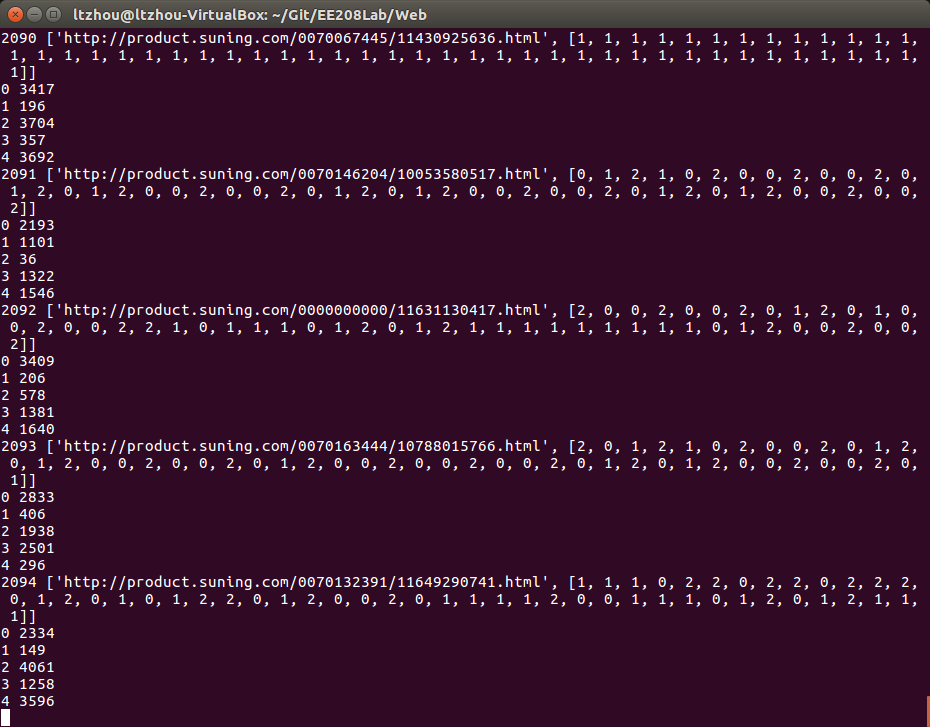
\includegraphics[width=13.5cm]{img/zlt/makehash.png}
\caption{建立哈希表}
\label{fig:makehash}   % 引用标记,用于文章中引用
\end{figure}